\documentclass[11pt,a4paper]{article}
\usepackage[margin=1in]{geometry}
\usepackage{amsmath, amssymb}
\usepackage{graphicx}
\usepackage{booktabs}
\usepackage{float}
\usepackage{hyperref}
\usepackage{subcaption}
\usepackage{setspace}

\hypersetup{
  colorlinks=true,
  linkcolor=blue,
  citecolor=blue,
  urlcolor=blue
}

\title{Finite-Population Rock--Paper--Scissors Dynamics}
\author{Ameer Alhashemi (2316492)}
\date{\today}

\begin{document}
\maketitle
\onehalfspacing

\begin{abstract}
In this report I implement and analyse a finite-population non-zero-sum Rock--Paper--Scissors (RPS) model using pairwise comparison (Local Update), a seasonal birth-only/death-only extension with fluctuating population size, and a creative network-based extension on a Watts--Strogatz small-world graph. For Question 1, I compare $s\in\{0.8,1.0,1.2\}$ and $w\in\{0.1,0.5,1.0\}$ with multi-seed summary statistics. For Question 2, I show that a slow seasonal forcing of birth probability produces large oscillatory fluctuations in $N(t)$ and I compare a baseline model to a mutation-robustness variant. For Question 3, I compare lattice and small-world dynamics and quantify how rewiring probability (hence clustering) affects coexistence drift. I discuss the results critically in relation to finite-size stochastic effects and established literature.
\end{abstract}

\section{Introduction}
Evolutionary game dynamics connects strategic interactions to stochastic population processes in finite systems. The required baseline here is a non-zero-sum RPS game under pairwise comparison (Local Update), where two agents are sampled and one may adopt the other's strategy with a probability increasing in payoff difference \cite{claussen2016,traulsen2006}. The assignment then asks for a model with separate birth and death events under seasonal forcing, and one creative extension (here: spatial/network interactions).

The payoff matrix used throughout is
\begin{equation}
A =
\begin{pmatrix}
0 & -s & 1 \\
1 & 0 & -s \\
-s & 1 & 0
\end{pmatrix},
\end{equation}
with $s>0$ controlling asymmetry and stability properties around the mixed state.

\section{Methods}
\subsection{Q1: Pairwise comparison in finite populations}
Population size is fixed at $N=150$. At each step, two distinct agents $A$ and $B$ are sampled uniformly. Each receives payoff against all other agents in the well-mixed population, and $B$ adopts $A$ with probability
\begin{equation}
p_{B\rightarrow A}
=
\frac{1}{2}
+
\frac{w(\pi_A-\pi_B)}{8\pi_{\max}},
\end{equation}
matching the Local Update form \cite{claussen2016}. I used
\begin{equation}
\pi_{\max}=(N-1)(1+s),
\end{equation}
as a bound on maximal possible payoff difference for this game. Initial conditions are near mixed equilibrium ($R,P,S$ approximately equal). I ran $T=30000$ steps for each parameter pair and used 20 random seeds for summary statistics. Required figures are generated as $R(t),P(t)$ time series and $(R,P)$ phase projections.

\subsection{Q2: Seasonal birth-only/death-only process}
To allow fluctuating population size, each step performs exactly one event:
\begin{itemize}
\item Birth-only event (probability $b(t)$): one sampled strategy replicates; opponent stays alive.
\item Death-only event (probability $1-b(t)$): one sampled agent dies.
\end{itemize}
The same pairwise comparison probability determines which sampled strategy is favored in birth or death selection. Seasonality is
\begin{equation}
b(t)=b_0 + a\sin(2\pi t/T_{\text{season}})
\end{equation}
with $b_0=0.50$, $a=0.30$, $T_{\text{season}}=8000$. I report:
\begin{enumerate}
\item baseline (no mutation),
\item robustness extension ($\mu=0.01$ mutation on birth).
\end{enumerate}
Plots show $R/N$, $P/N$, and scaled $N(t)$.

\subsection{Q3: Creative extension (lattice and small-world)}
I implemented two spatial/network variants:
\begin{enumerate}
\item 2D periodic lattice (von Neumann neighborhood, degree 4);
\item Watts--Strogatz small-world network with degree $k=8$ and rewiring $\beta\in\{0,0.1,0.5\}$ \cite{watts1998}.
\end{enumerate}
Update is again pairwise Local Update on links. For network comparability across rewiring levels, payoffs are degree-normalized (average payoff per neighbor) so observed effects are less confounded by degree heterogeneity. I measured clustering coefficient $C$ and late-time distance to mixed point
\begin{equation}
d(t)=\sqrt{(R/N-1/3)^2+(P/N-1/3)^2}.
\end{equation}

\section{Results}
\subsection{Q1 parameter comparison}
Table~\ref{tab:q1} summarizes median extinction times (first time at least one strategy count hits zero), which is a practical finite-population stability proxy.

\begin{table}[H]
\centering
\caption{Q1 summary over 20 seeds per parameter pair ($N=150$, $T=30000$).}
\label{tab:q1}
\begin{tabular}{cccc}
\toprule
$s$ & $w$ & Median first-extinction time & Mean first-extinction time \\
\midrule
0.8 & 0.1 & 9069.0 & 11234.6 \\
0.8 & 0.5 & 11194.5 & 12487.8 \\
0.8 & 1.0 & 16848.0 & 17911.1 \\
1.0 & 0.1 & 10534.5 & 11868.0 \\
1.0 & 0.5 & 8426.0 & 9609.7 \\
1.0 & 1.0 & 12563.5 & 12806.6 \\
1.2 & 0.1 & 10534.5 & 11352.6 \\
1.2 & 0.5 & 10206.5 & 10883.6 \\
1.2 & 1.0 & 11383.5 & 12395.3 \\
\bottomrule
\end{tabular}
\end{table}

Observed dependence on $w$ and $s$ is non-monotone in finite populations, consistent with strong stochastic effects and trajectory variability. A single-seed interpretation would be misleading; multi-seed statistics are necessary.

\begin{figure}[H]
\centering
\begin{subfigure}[t]{0.48\textwidth}
  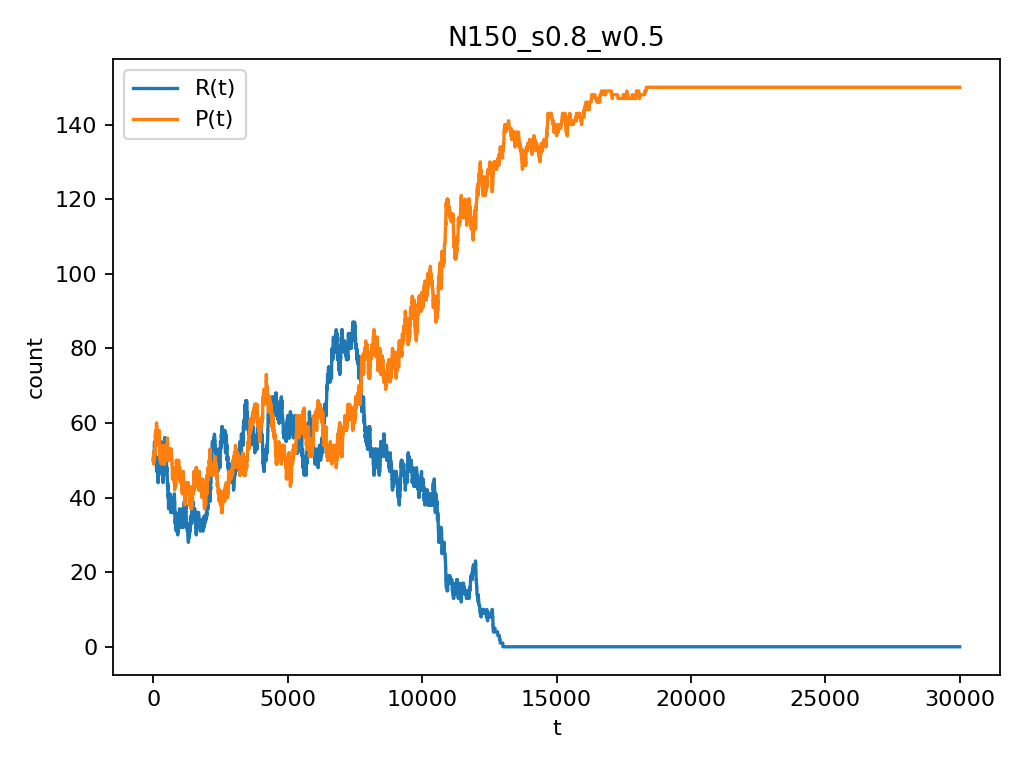
\includegraphics[width=\textwidth]{results/N150_s0.8_w0.5_timeseries.png}
  \caption{$s=0.8,\;w=0.5$}
\end{subfigure}
\hfill
\begin{subfigure}[t]{0.48\textwidth}
  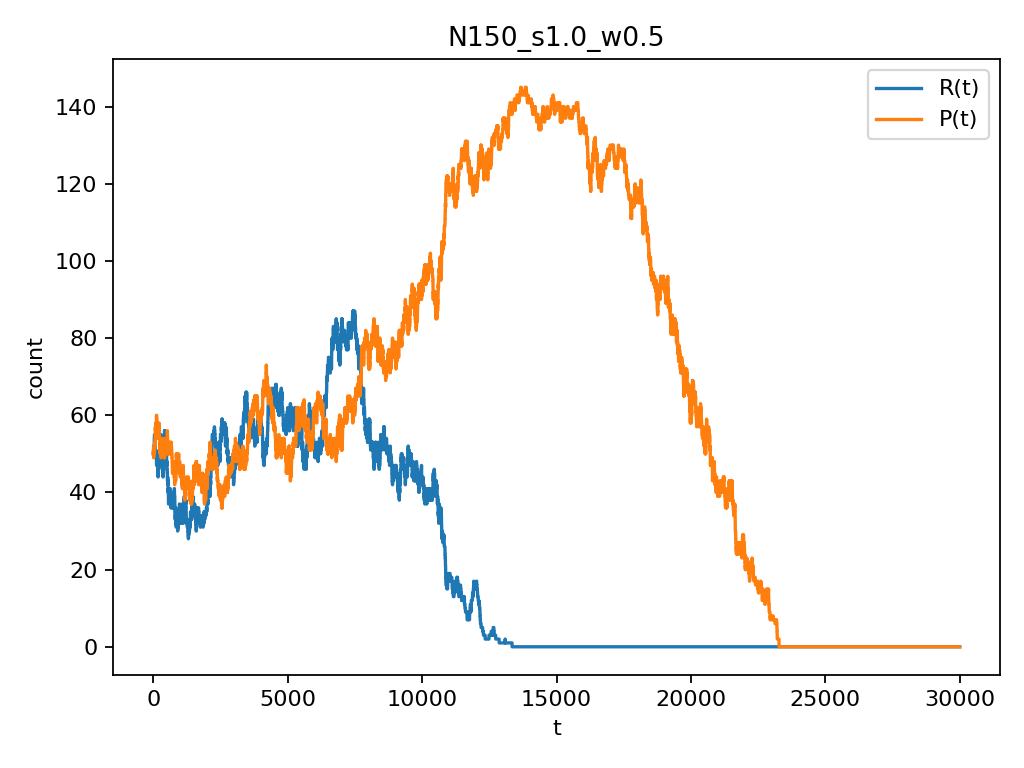
\includegraphics[width=\textwidth]{results/N150_s1.0_w0.5_timeseries.png}
  \caption{$s=1.0,\;w=0.5$}
\end{subfigure}
\caption{Representative Q1 time series (single seed, used only as trajectory examples).}
\label{fig:q1-timeseries}
\end{figure}

\subsection{Q2 seasonal fluctuating population}
Table~\ref{tab:q2} shows strong fluctuation between small and large $N$ in both variants.

\begin{table}[H]
\centering
\caption{Q2 means over 10 seeds per variant ($T=40000$).}
\label{tab:q2}
\begin{tabular}{lccccc}
\toprule
Variant & Mean $N_{\min}$ & Mean $N_{\max}$ & Mean $\bar N$ & Mean $N_{\text{last}}$ & Mean extinct-steps \\
\midrule
Baseline ($\mu=0$) & 50.1 & 1792.5 & 927.8 & 186.4 & 4031.8 \\
Mutation ($\mu=0.01$) & 54.5 & 1763.1 & 907.6 & 180.1 & 704.5 \\
\bottomrule
\end{tabular}
\end{table}

Mutation substantially reduces extinction episodes but does not remove large $N$ oscillations. Thus, the seasonal birth/death forcing is the dominant driver of population-size fluctuations.

\begin{figure}[H]
\centering
\begin{subfigure}[t]{0.48\textwidth}
  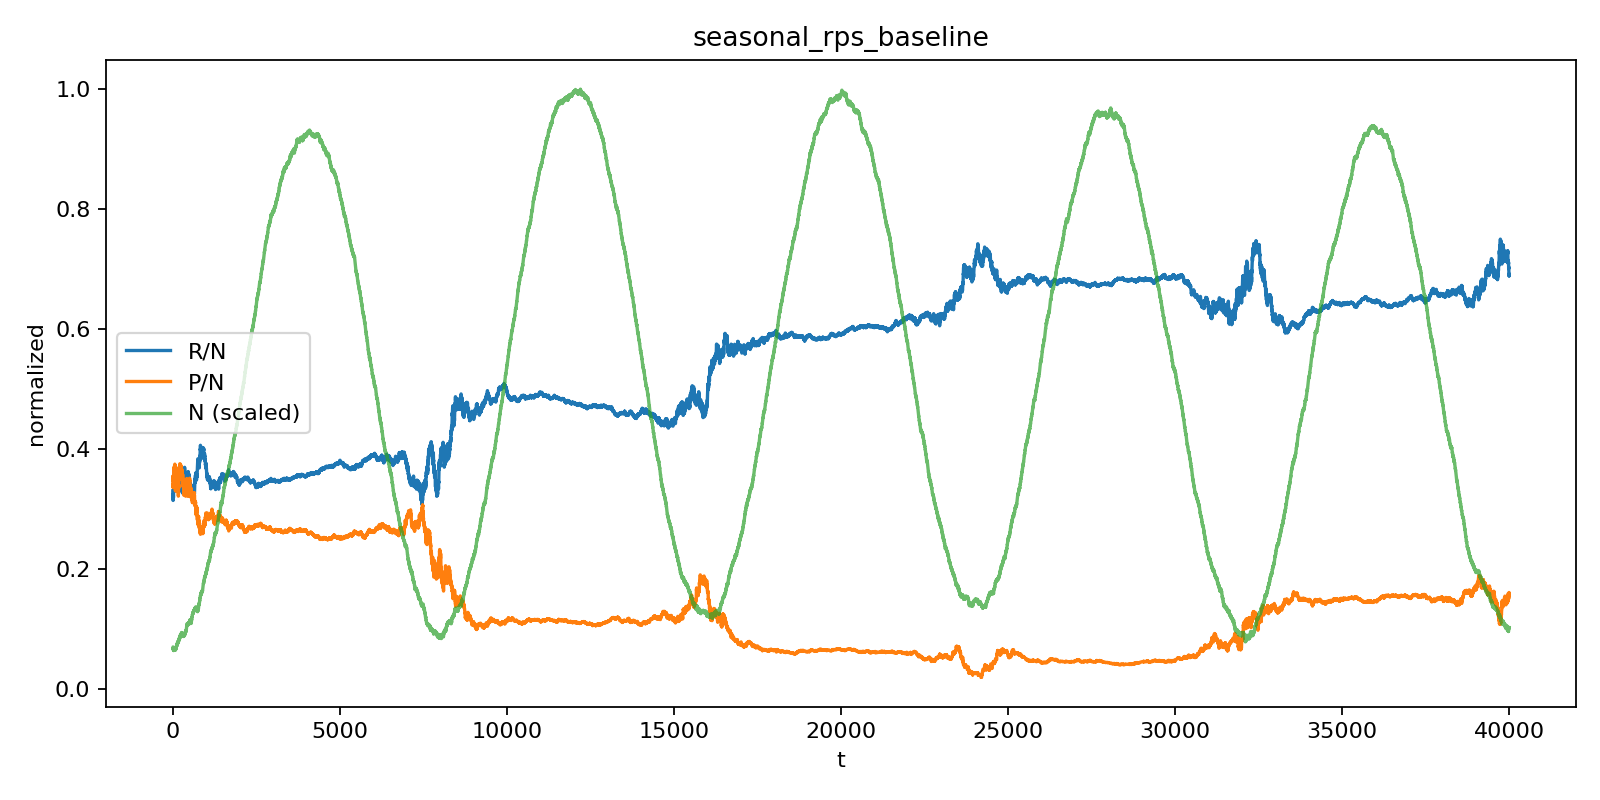
\includegraphics[width=\textwidth]{results_q2/seasonal_rps_baseline_timeseries.png}
  \caption{Baseline ($\mu=0$)}
\end{subfigure}
\hfill
\begin{subfigure}[t]{0.48\textwidth}
  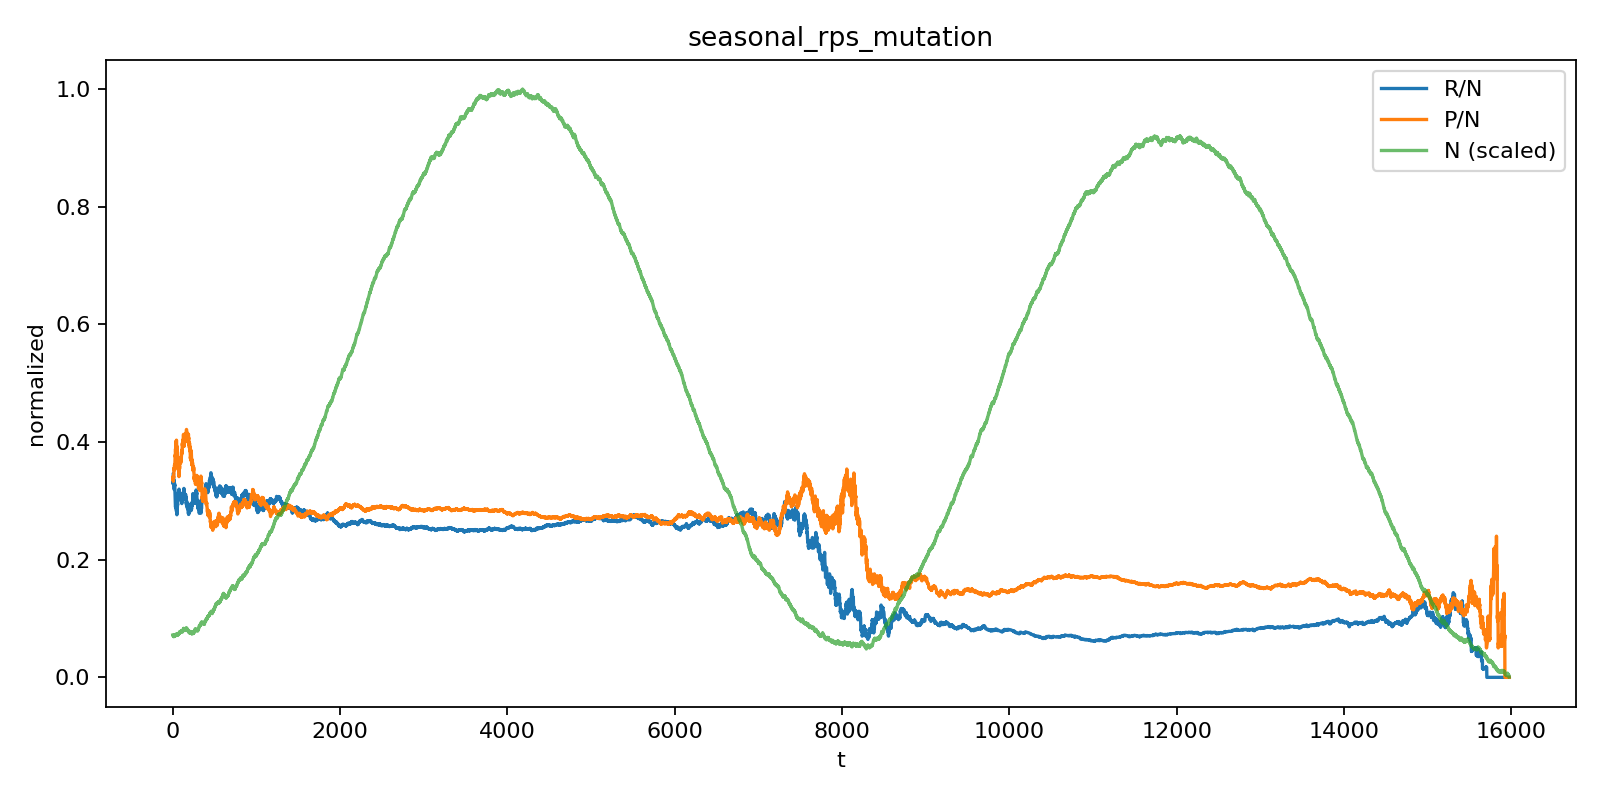
\includegraphics[width=\textwidth]{results_q2/seasonal_rps_mutation_timeseries.png}
  \caption{Mutation extension ($\mu=0.01$)}
\end{subfigure}
\caption{Q2 seasonal model: normalized composition and scaled $N(t)$.}
\label{fig:q2-timeseries}
\end{figure}

\subsection{Q3 creative extension: lattice vs small-world}
For the lattice ($L=40$, $N=1600$), averaged over 8 seeds:
\[
\overline{d}_{\text{late}} = 0.0836,\quad
(\bar R,\bar P,\bar S)=(0.3216,0.3600,0.3184).
\]

For the small-world model, Table~\ref{tab:q3sw} reports seed-averaged outcomes.

\begin{table}[H]
\centering
\caption{Q3 small-world means over 8 seeds per $\beta$ (degree-normalized payoff).}
\label{tab:q3sw}
\begin{tabular}{ccccc}
\toprule
$\beta$ & Mean $C$ & Mean late $d$ & Mean final $(R,P,S)$ \\
\midrule
0.0 & 0.6429 & 0.0322 & (0.3487, 0.3190, 0.3323) \\
0.1 & 0.4699 & 0.0480 & (0.3212, 0.3437, 0.3352) \\
0.5 & 0.0854 & 0.0580 & (0.3220, 0.3441, 0.3339) \\
\bottomrule
\end{tabular}
\end{table}

Higher rewiring (lower clustering) tends to increase late-time distance from the mixed point in this setup, though variability across seeds remains non-negligible.

\begin{figure}[H]
\centering
\begin{subfigure}[t]{0.32\textwidth}
  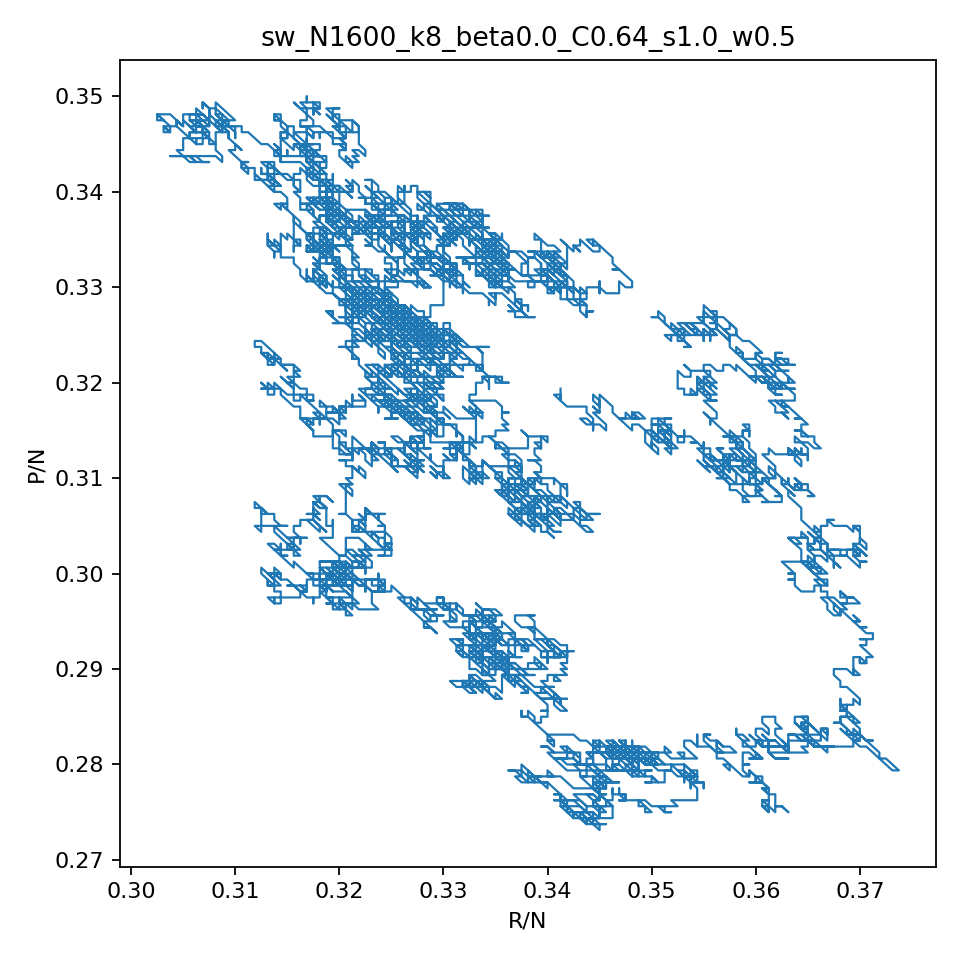
\includegraphics[width=\textwidth]{results_q3_sw/sw_N1600_k8_beta0.0_C0.64_s1.0_w0.5_phase.png}
  \caption{$\beta=0.0$}
\end{subfigure}
\hfill
\begin{subfigure}[t]{0.32\textwidth}
  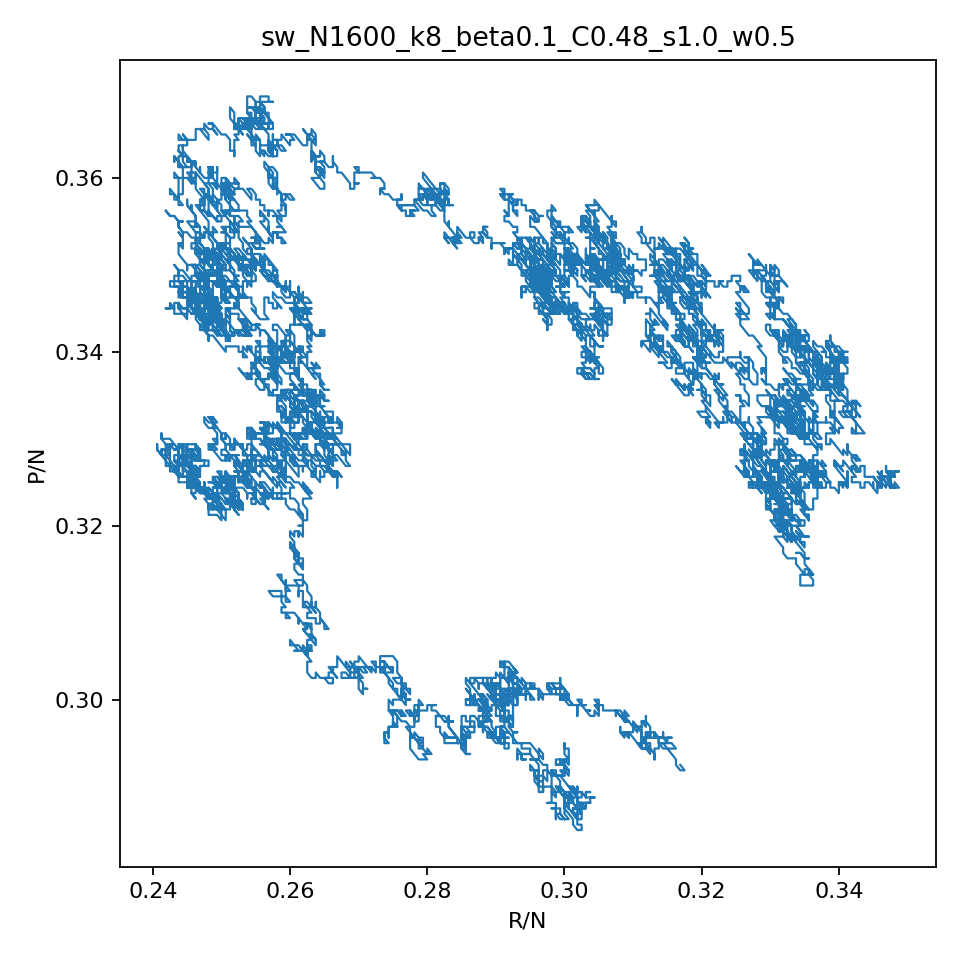
\includegraphics[width=\textwidth]{results_q3_sw/sw_N1600_k8_beta0.1_C0.48_s1.0_w0.5_phase.png}
  \caption{$\beta=0.1$}
\end{subfigure}
\hfill
\begin{subfigure}[t]{0.32\textwidth}
  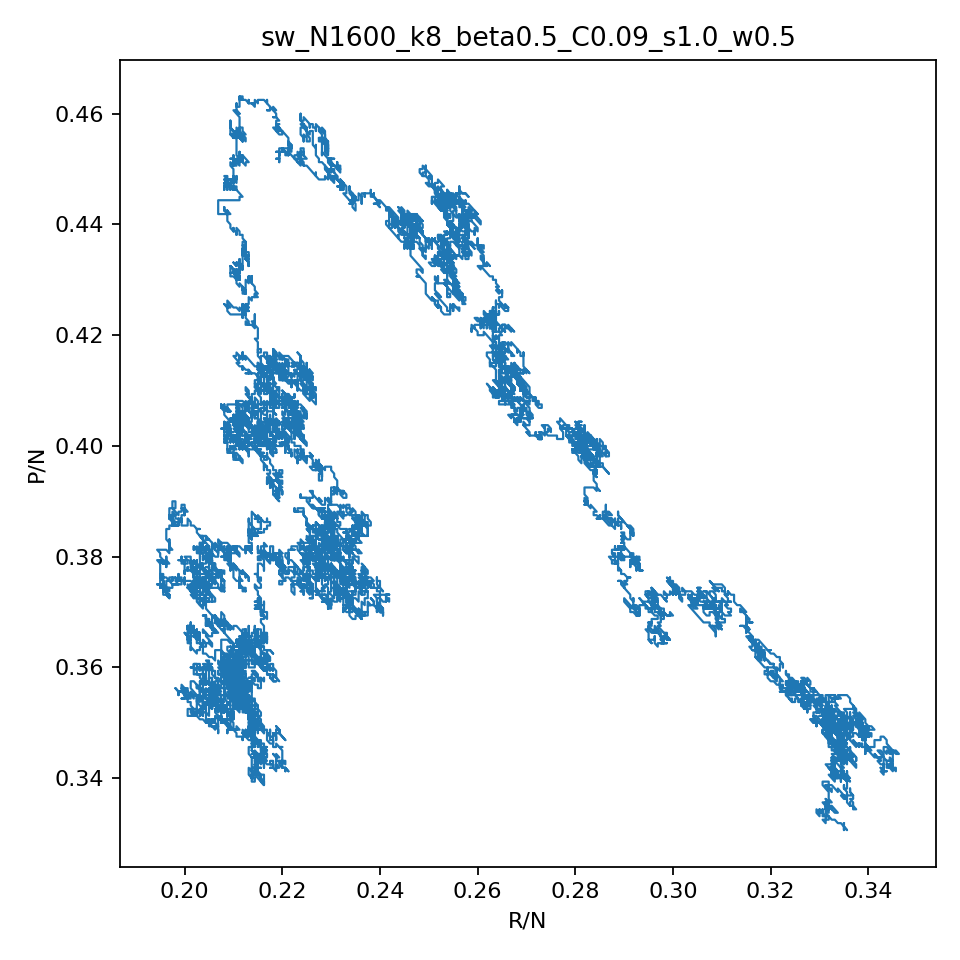
\includegraphics[width=\textwidth]{results_q3_sw/sw_N1600_k8_beta0.5_C0.09_s1.0_w0.5_phase.png}
  \caption{$\beta=0.5$}
\end{subfigure}
\caption{Q3 small-world phase plots for three rewiring levels.}
\label{fig:q3-sw-phase}
\end{figure}

\section{Discussion and Critical Reflection}
Overall, the implementation satisfies the three assignment components and produces coherent dynamics across well-mixed, seasonal, and networked settings. The strongest practical lesson from my results is that finite-size stochasticity is not a minor detail: it materially changes the apparent stability story compared with deterministic intuition. This is clearest in Q1, where the qualitative behavior can look different across seeds even for the same parameters, which means conclusions should rely on distributions (or at least repeated runs) rather than a single trajectory. In Q2, the model succeeds in creating pronounced population-size variation between small and large $N$, but the exact timing and depth of low-$N$ intervals remain sensitive to parameterization of the seasonal forcing, so interpretation should focus on robust patterns (e.g., sustained fluctuations and extinction pressure) rather than on individual transient episodes. In Q3, the lattice and small-world results show that structure matters, but they also highlight that network conclusions depend on update design choices such as payoff normalization and the observation window; this makes it important to avoid over-generalizing from one network construction or one time horizon. A reasonable next step would be to add confidence intervals for all key summary metrics and test an additional update rule (such as Fermi updating) to see which conclusions are process-specific versus structurally robust.

\section{Conclusion}
This coursework reproduces finite-population RPS dynamics under Local Update, extends to seasonally fluctuating birth/death with variable population size, and explores spatial/network effects in a creative extension. The main practical takeaway is that finite stochasticity and update-process details materially affect apparent stability/coexistence, so robust multi-seed analysis is necessary before drawing conclusions.

\section*{Acknowledgements and Source Statement}
All code and analysis in this submission were prepared by Ameer Alhashemi. External sources used for model specification and interpretation are cited in this report and acknowledged in the script headers.

\bibliographystyle{plain}
\bibliography{references}

\end{document}
